\chapter{Hardware design of a low-cost sensor node}\label{chap3}

We use low-cost sensors we designed to detect on-off state change on each appliance, and to report to the single base station. The sensor plugs in an AC outlet, and provides one AC outlet for the appliance. Each appliance in question should connect to a separate sensor directly. Hence, an important design goal is low-cost. And we achieve the goal not by choosing cheap components, but simplifying the functionality. The extremely low price is inherent in the simplicity. 

%"Simplicity is the ultimate sophistication." - Leonardo Da Vinci

The functions and design goals of the sensor are
\begin{itemize}
  \item Detect binary (on-off) state changes
  \item Reliably deliver detected events to a central node
  \item Low cost
\end{itemize}

The overall block diagram of the sensor hardware is shown in Fig.\ref{fig:hwoverview}. And Fig.\ref{fig:sensor} is a photo of our prototype. 

\begin{figure}[htb]
  \centering
  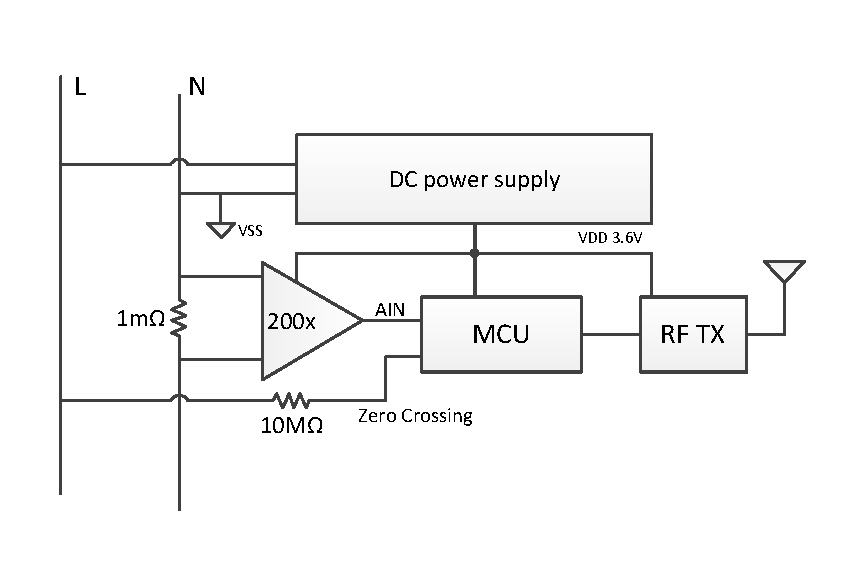
\includegraphics[width=0.8\textwidth]{figures/hwoverview}
  \caption{Block diagram of the on-off state sensor hardware}
  \label{fig:hwoverview}
\end{figure}

\begin{figure}[htb]
  \centering
  \includegraphics[width=0.6\textwidth]{figures/nilmbee2}
  \caption{Photo of the sensor prototype}
  \label{fig:sensor}
\end{figure}

\section{On-off state sensing}

As discussed before, one of the function of the sensor is to detect binary (on-off) state changes. Typically, in order to get instantaneous power, both voltage and current need to be sampled, and they are multiplied and accumulated. The power calculation is usually done in a separate metering chip, or as a separate module integrated in a microcontroller. In our design, we choose to sample the current only, and detect state change solely based on the change of current. Although there is not enough information to obtain the actual power consumption from the current, our experiments show that it is enough to detect on-off events. In this way, the circuitry can be simpler without the voltage channel and the dedicated metering chip. 

A $1m\Omega$ resistor in series captures the instantaneous current flow. The voltage drop across the resistor is amplified 100 times by two stages of amplifier. An ATTiny10 microcontroller then samples the signal at approximately 1.6kHz, and run the event detection algorithm. 

The event detection algorithm run on the microcontroller is shown in fig \ref{fig:eventdetect}. Firstly, the range (i.e. $max - min$) of instantaneous current signal is taken for each 200-sample window. Note that the range is not necessarily the peak-peak amplitude of the signal, due to clippings discussed later. Nevertheless, the range do captures enough information for on-off state detection. Then, we take a threshold and get an instantaneous binary state for each window. Note that the threshold is adjusted slightly based on the state of the appliance, so that the binarization has some hysteresis. 

\begin{figure}[htb]
  \centering
  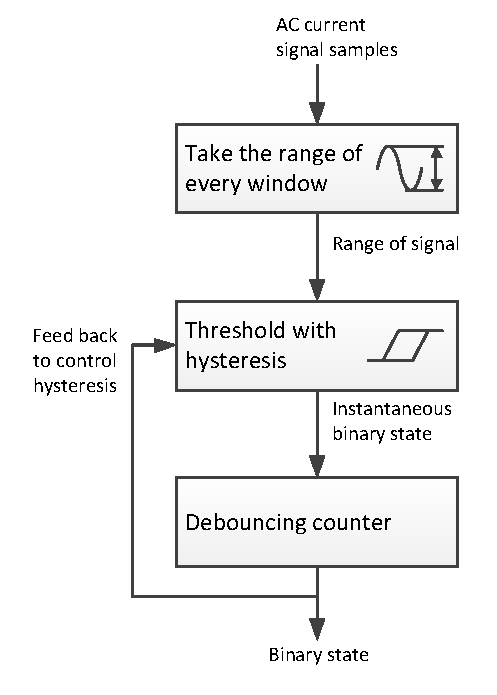
\includegraphics[width=0.5\textwidth]{figures/eventdetect}
  \caption{Event detection algorithm flowchart}
  \label{fig:eventdetect}
\end{figure}

The threshold is hardcoded in the microcontroller firmware, and it is set to around 5W. Appliances with dry-contact switch, such as lamps and lights, draw absolutely zero power when turned off. Other appliances with soft-controlled switch, such as microwave and computer monitors, draw a very low standby power when turned off. Our experiments show that 5W is a reasonable threshold for most appliances. 

The window in which the range of samples is taken and binarized is about 12ms, or about 7 AC cycles long. The length ensures quick response to state changes, but the instantaneous state is too sensitive and bouncing. Therefore, we employ a debouncing counter that counts up to 16. Then appliance state is changed only when 16 successive windows all show the opposite state. 

As mentioned before, the range of samples in each window not necessarily represents the peak-peak amplitude. The reason is as following. Both the amplifier and the ADC are powered with a single positive DC power. Ideally, the negative half of the AC signals will be clipped in all stages of amplification and AD conversion. In the real circuit, some Op-Amps we use may have negative input bias voltage up to -4mV. To compensate it, we use a $2.4M\Omega$ pull-up resistor to bias the input signal. 

Although the analog front-end is not designed to reduce noise and best preserve the signal, it is good enough for detecting binary states. 

\section{Unidirectional radio}

The sensor should be able to transmit detected events to a central base station. There are several technologies for networking sensor nodes in short ranges. For instance, IEEE 802.15.4 is a standard for short range radio communication, and is widely used in sensor networking. Proprietary wireless sensor network technologies are also available such as ANT radio and TI sub-GHz radio. On the other hand, communication is also possible through the AC power lines, namely Power-line Communication (PLC). The most popular PLC technology for home automation is X10, despite its low bitrate. 

We do not use the most popular wireless sensor network radio technologies such as 802.15.4, because it is an overkill. These radio technologies usually provide several hundred kBps or even several MBps of duplex link, with sophisticated packeting and MAC, etc. These radio ICs are a few dollars each. In order to control the radio chip, microcontroller needs to have SPI or other serial link, which further pushes up the requirement of the microcontroller, as well as the price. However, in our case, appliances usually generate events once per several minutes, or even hours. And a state changing event is literally one bit of data, plus the ID of sensors and few control bits. 

Low rate PLC technology is suitable for our application. However, it is not low cost enough, and has other problems inherently. To couple signals onto the power lines, PLC transmitter needs coils which are costly and big in size. Appliances can insert interferences on the power lines, making the channel even worth than wireless channels. Moreover, devices on different circuits can not communicate without a bridge device. 

Considering our requirements, we decide to use a bare-bone 315MHz ASK transmitter. The transmitter module is basically a oscillator, with one pin controlling its on or off. We designed a coding scheme (details in Appendix \ref{app1}). And because it is transmit-only, to improve reliability, we designed a retransmission scheme, which will be discussed in detail in Chapter \ref{chap4}. 

\section{DC Power supply}

The sensor draws power from AC power lines with a voltage-drop-capacitor DC power supply. This is a DC supply topology with very compact design and low cost, suitable for low current DC requirements. The supply voltage of the circuit is 3.6V DC with the neutral line as reference voltage. The current is 3mA when standby, 15mA when transmitting. 

We also have zero-crossing detection in our circuit, used for synchronization and timing purposes. 

\section{Cost and scalability}

There are several design decisions that make the sensor inherently inexpensive. By sensing the current, instead of power, we eliminate the need for a meter IC or a microcontroller with meter module. Because only a binary output is needed, distortion and clippings are tolerable. Thus, we do not need to calibrate the analog frontend. By employing a simple RF module, we eliminate the need for an RF IC or a microcontroller with SPI or other interfaces. 

Without the need for any peripherals other one analog input and two digital GPIOs, we are able to use the simplest microcontrollers. The microcontroller we use in our design is ATtiny10, which is a 6-pin chip. Nevertheless, the functions of the microcontroller are merely taking threshold and smooth it, and toggle a pin for RF transmission. The first two can be done with pure analog circuitry, while the latter can be replaced by a sequence generator circuitry. Hence, it is even possible to replace the microcontroller with a very simple customized IC, which is more cost-effective at very large quantity. 

We reuse the plastic packaging of a commercial plug-load timer to make our prototype sensors, as shown in Fig.\ref{fig:sensor}. Hence, the physical size is limited by the packaging. In fact, the circuit board can be made much smaller. It is even possible to include the circuitry in every plug or every outlet. The cost of all components of our prototype board is 2.3 US dollars each at a quantity of 1000. Combined with the PCB and packaging and assembly, the overall cost should be as low as 4.3 US dollars. It is totally affordable to have one sensor for each appliance, considering that appliances are usually tens or hundreds of dollars. 

